\documentclass{article}
\usepackage[utf8]{inputenc}
\usepackage[tmargin=1in,bmargin=1in,lmargin=1.25in,rmargin=1.25in]{geometry}
\usepackage{graphicx}
\usepackage{float}
\usepackage{parskip}
\renewcommand{\familydefault}{\sfdefault}
\usepackage{hyperref}
\hypersetup{
    colorlinks,
    citecolor=black,
    filecolor=black,
    linkcolor=black,
    urlcolor=black
}

\begin{document}

\begin{titlepage}
    \begin{center}
        \vspace*{1cm}
        \Huge
        \textbf{Grey JCR Website Manual}
        \\
        \vspace{1cm}
        \LARGE
        \textbf{January 2021}
        \vfill
        
\includegraphics[width=0.4\textwidth]{logo512.png}
    \end{center}
\end{titlepage}

\newpage
\tableofcontents
\newpage

\section{Election System}
Last updated: 25/01/2021

To use the election system you will require the permission 'Manage Elections'. Anybody with this permission will be able to create, edit, delete, generate results, and see in-depth anonymous voting logs for each election. It is strongly advised that you manage elections on a computer using Google Chrome or Microsoft Edge (soon to also support Safari once the next update from Apple is live) rather than mobile for a more consistent experience To begin managing the elections you will need to login to the website and, if you have the correct permissions, you will see 'Admin Options' in the navigation bar. Hover over this to activate the drop-down and click 'Manage Elections'.
\subsection{Create a New Election}
From the main election management page, click the green button 'Create New Election' to open the separate page that allows you to create a new election. Initially the page will look like this:
\begin{figure}[H]
    \centering
    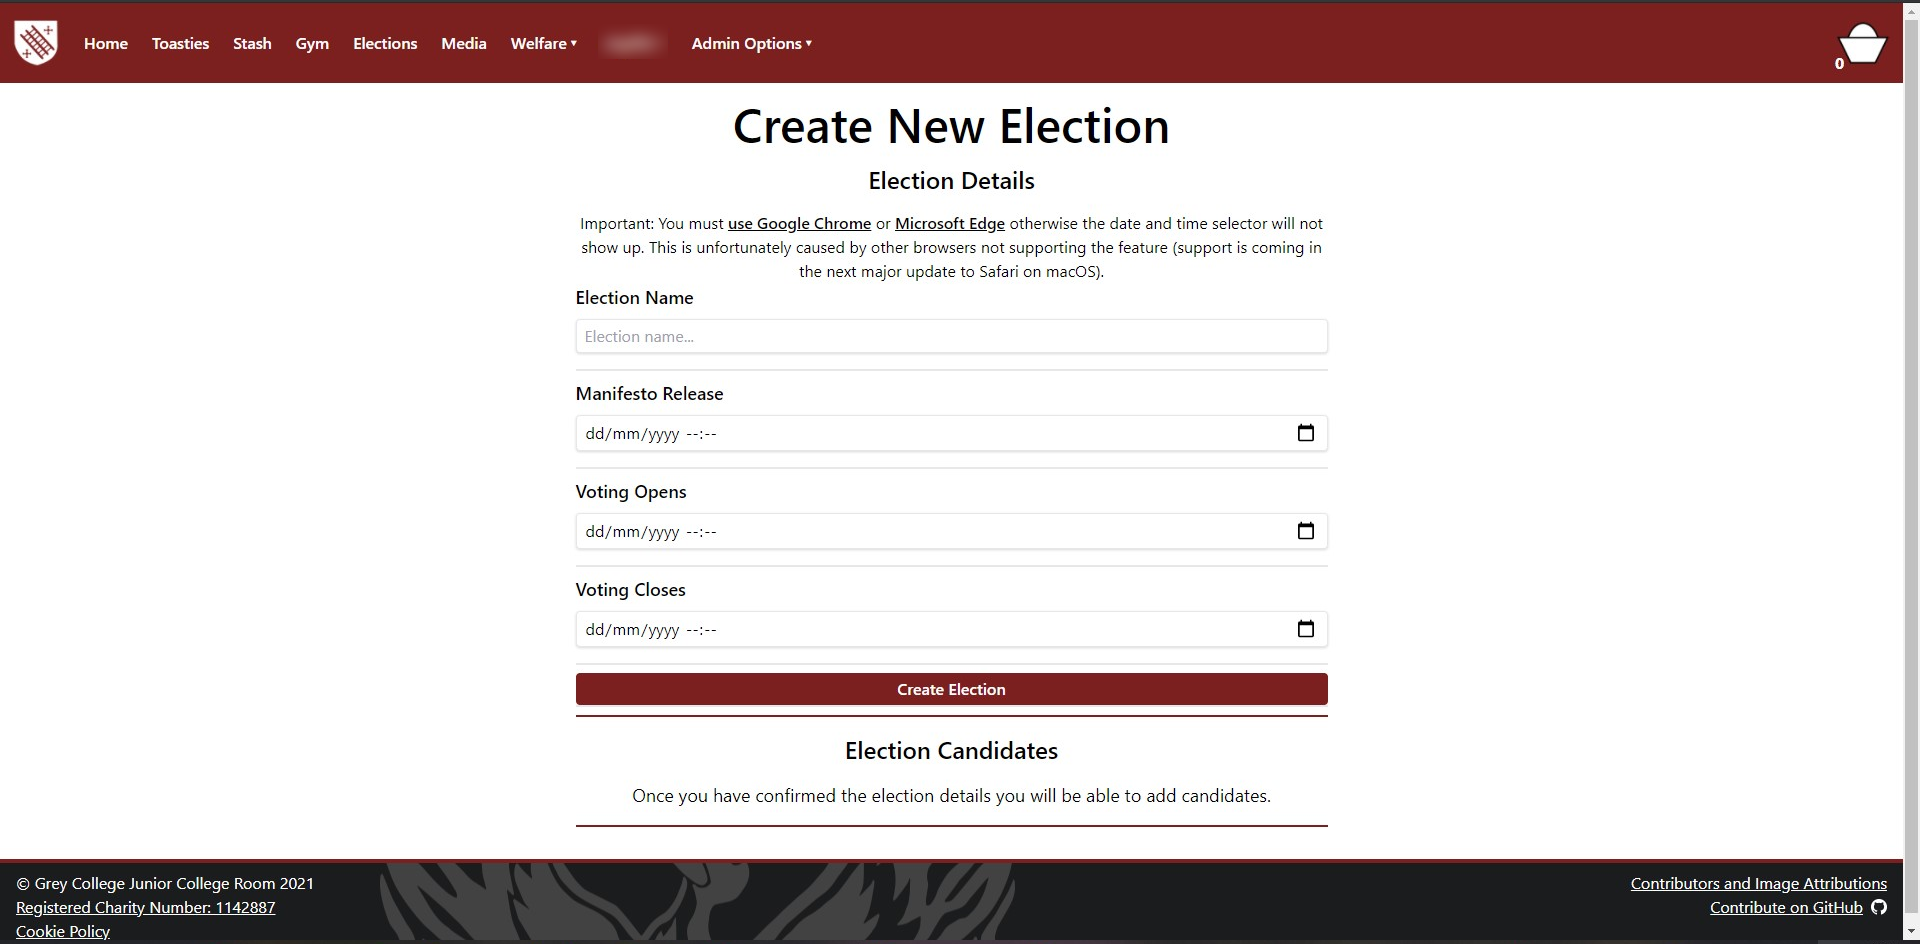
\includegraphics[width=\textwidth,height=\textheight,keepaspectratio]{elections/initial_create_screen.png}
    \caption{Election Creation: Add Details}
    \label{fig:election_creation_start}
\end{figure}
The initial steps are:
\begin{enumerate}
    \item Type the name of the election in the 'Election Name' text field
    \item Select a date and time for the release of the manifestos (Warning: If you are not using Chrome or Edge this may appears as blank text field like the election name field. You will need to type the date-time in the format yyyy-MM-dd hh:mm:ss)
    \item Select a date and time for when the voting will open. This must be after the manifesto release.
    \item Select a date and time for when the voting will close. This must be after the voting opens.
\end{enumerate}
Once you are happy with these details click 'Create Election'. You can edit these details later if necessary (see the next subsection). The screen will change slightly now. At the top you will find the confirmed details for the election you have created. Now you can begin adding candidates.
\begin{figure}[H]
    \centering
    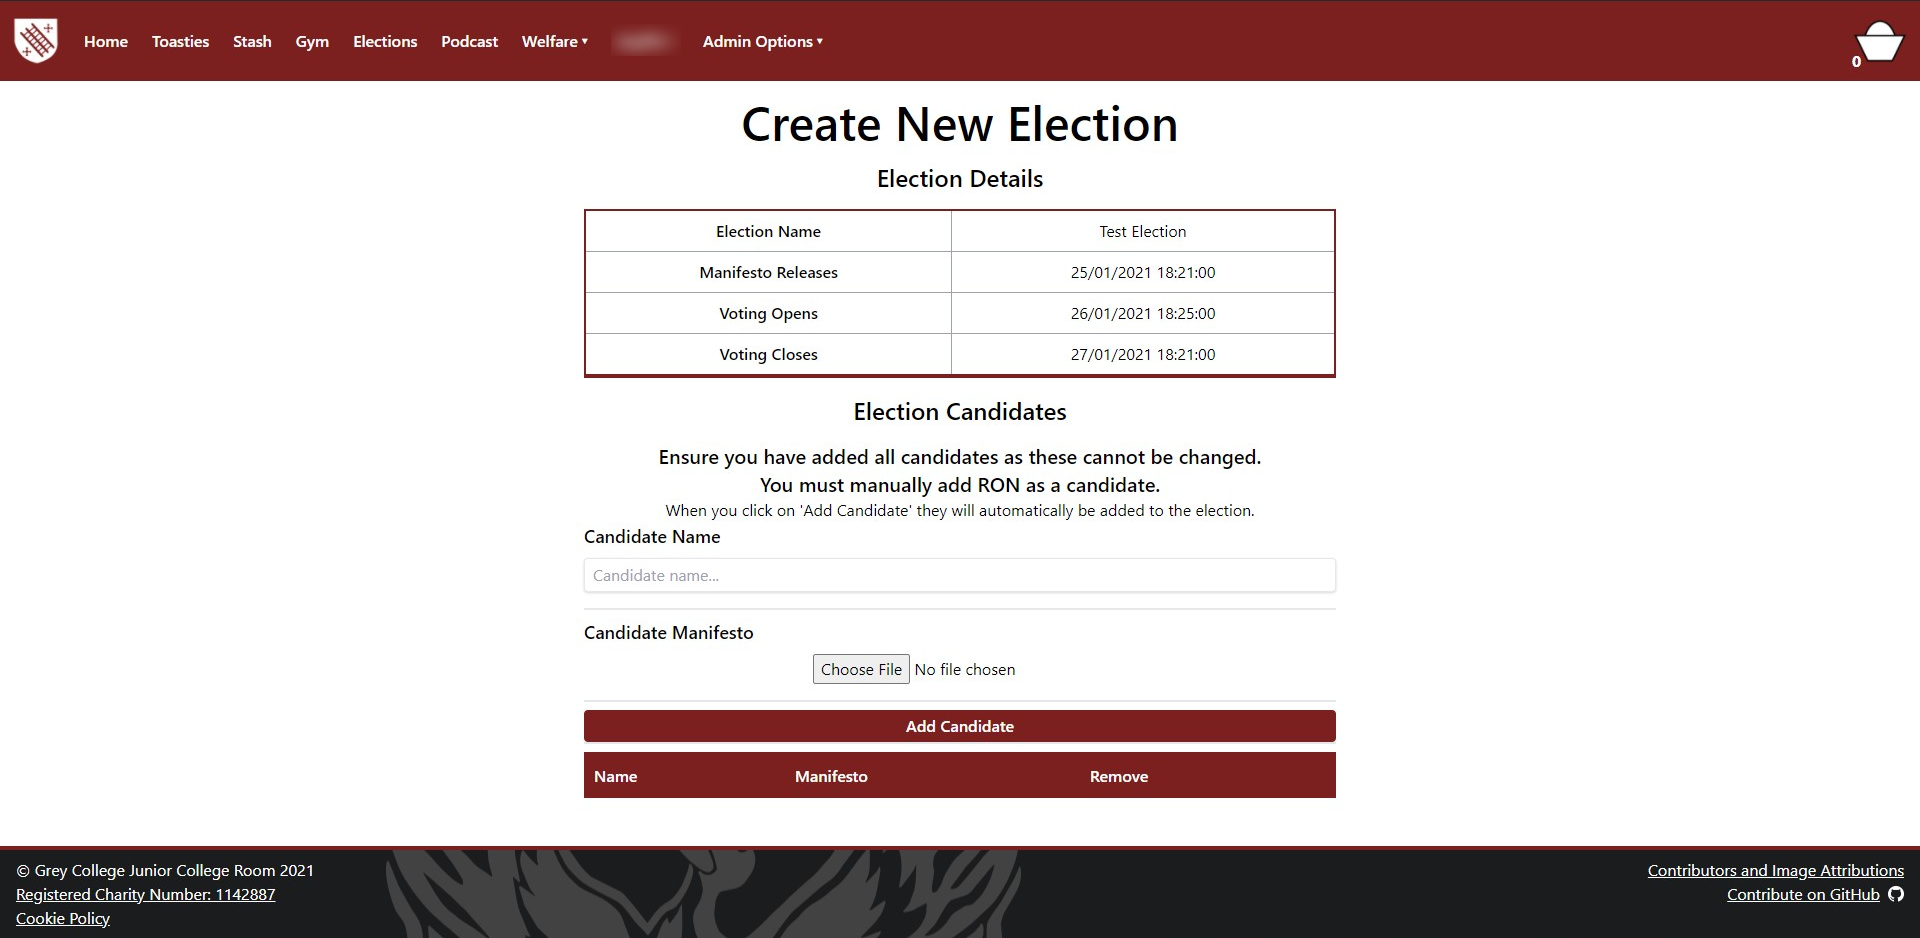
\includegraphics[width=\textwidth,height=\textheight,keepaspectratio]{elections/add_candidate_screen.png}
    \caption{Election Creation: Add Candidates}
    \label{fig:election_add_candidate}
\end{figure}
\textbf{It is important to note that candidates and their manifestos cannot be edited once you leave this page!} (Note for Website Editor: Although if something urgently needs changing you can make these changes manually by editing the tables 'Elections' and 'ElectionCandidates'.)
\\[12pt]
To add a new candidate:
\begin{enumerate}
    \item Type their name in the 'Candidate Name' text field
    \item Then click the 'Choose File' button and select their manifesto
    \item Click 'Add Candidate'
\end{enumerate}
Repeat this process for each candidate. \textbf{The system does not automatically add RON, you will need to manually do this each time you make a new election} (this is intentional as the election system may be used for other votes such as referendums). Once you have added every candidate you can simply leave the page. Your changes are saved each time you add/remove a candidate automatically. 
\subsection{Edit an Election}
Once you have created an election you can then edit the name, manifesto release date, voting opening date and voting closing date. Any changes you make will be logged and you must type a reason as to why you have made such a change to ensure that elections are transparent. To access this page click the 'Edit' button on the row of the table representing the election you are interested in. Once you click this you will be taken to a separate page.
\begin{figure}[H]
    \centering
    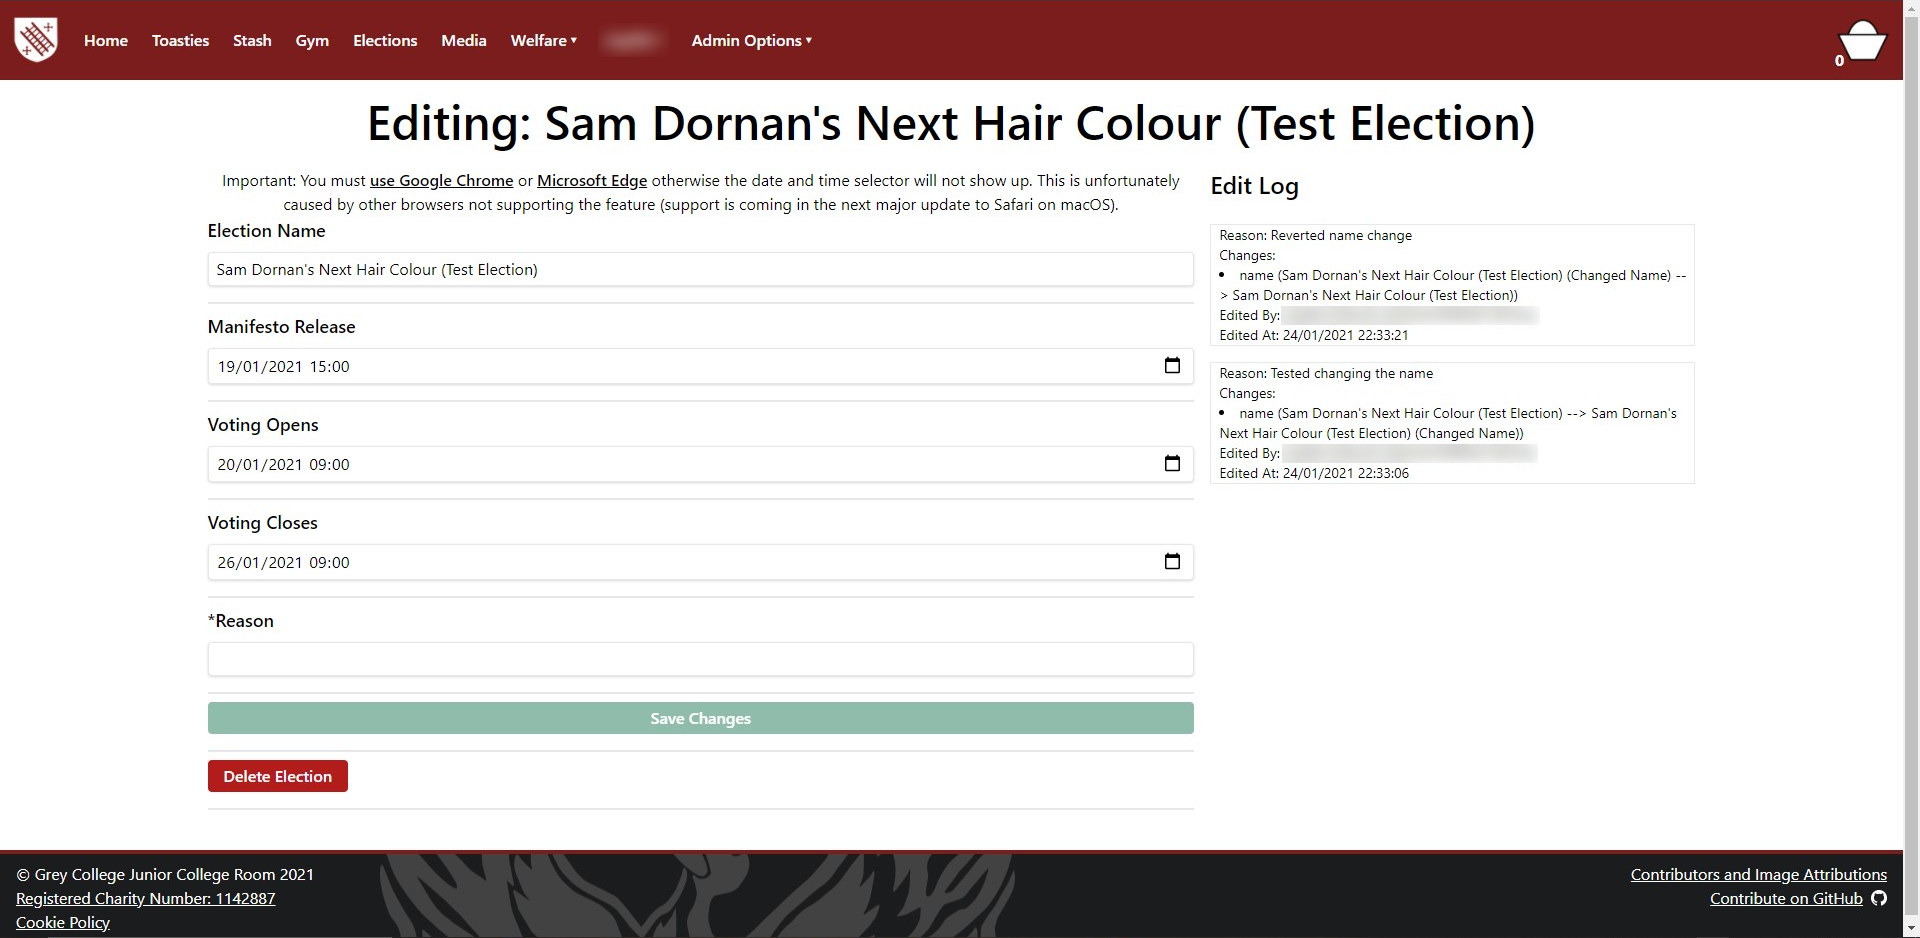
\includegraphics[width=\textwidth,height=\textheight,keepaspectratio]{elections/election_edit.png}
    \caption{Election Edit Page}
    \label{fig:election_edit}
\end{figure}
On the left hand side is the fields that can be edited. The same conditions apply to the dates (manifestos release before voting opens which opens before voting closes). On the right hand side you can see the edit log.

At the bottom of the page is a 'Delete Election' button. This should only be used in extreme cases (e.g. needing to change candidates). Pressing the button will purge all of the related manifestos, candidates and votes for that election. When you do this the JCR President, FACSO, and Chair will receive an email notifying them that the election has been deleted as well as the name and username of the person who deleted it.
\subsection{Results}
\subsubsection{Generating the Results}
Once an election has concluded you will be able to generate the results from the management page. \textbf{Please note that once you generate the results you will no longer be able to edit the election. This includes extending the voting deadline.} (Note for Website Editor: If necessary, you can delete the contents in the fields 'winner', 'deepLog', 'roundSummaries' and 'published' fields in the 'Elections' table to allow changes to be made.) On the management page, the row related to the election will look like so:
\begin{figure}[H]
    \centering
    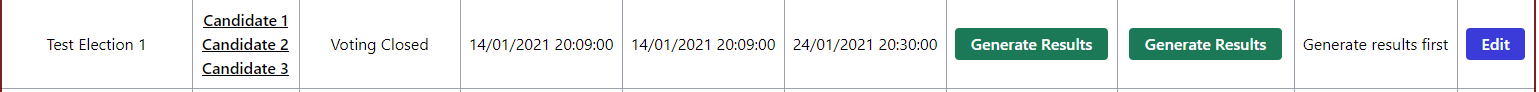
\includegraphics[width=\textwidth,height=\textheight,keepaspectratio]{elections/election_row_generate.png}
    \caption{Election row ready for result generation}
    \label{fig:election_generation_ready}
\end{figure}
Click either of the large green buttons 'Generate Results'. This will redirect you. It may take a little while to compute the results depending on the turnout for the vote. At the time of writing this we have not had a large scale test of the results generation but it should take less than a minute to produce the results for you. Once the results have been generated you will see a screen like this:
\begin{figure}[H]
    \centering
    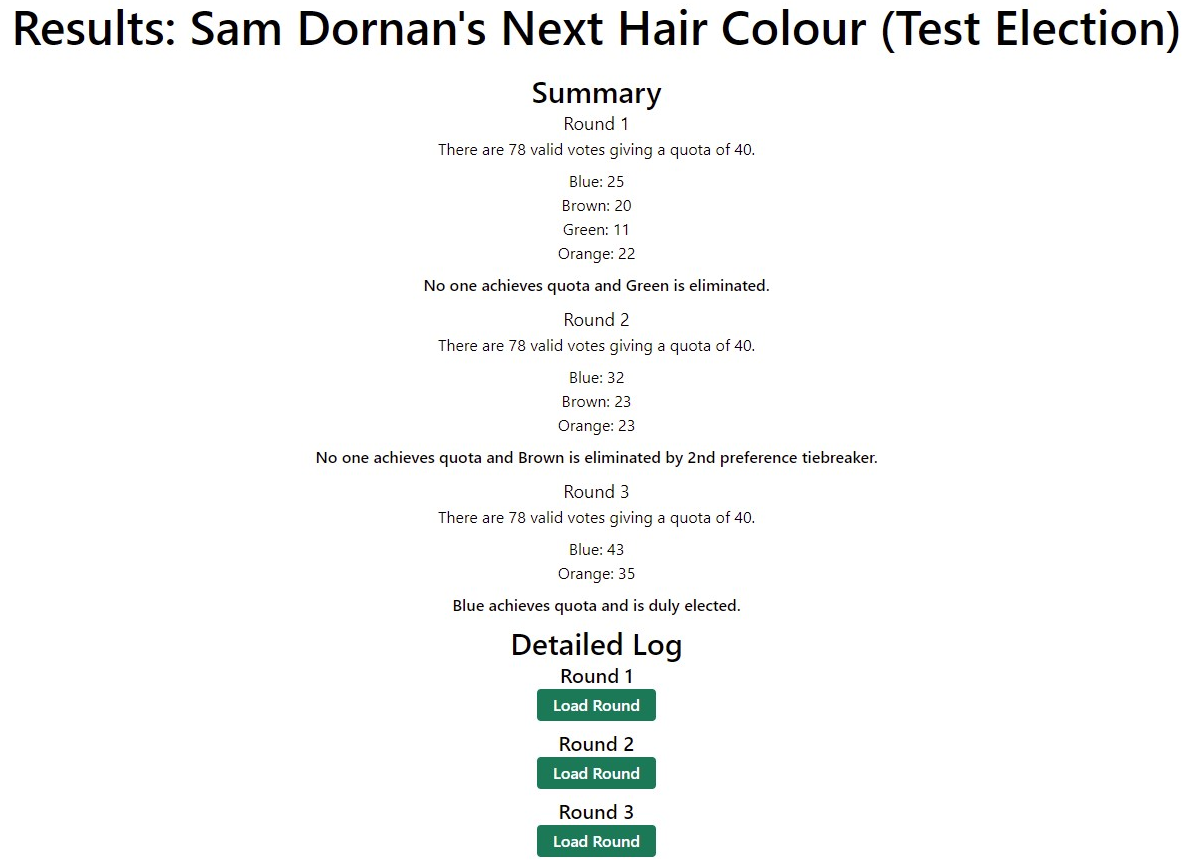
\includegraphics[width=\textwidth,height=\textheight,keepaspectratio]{elections/election_results.png}
    \caption{Election results after generation}
    \label{fig:election_results_generated}
\end{figure}
\subsubsection{Interpreting the Results}
This will summarise all of the information about the election. The are a few potential cases that could arise:
\begin{itemize}
    \item {[Candidate Name]} achieves quota and is duly elected: This means the person was elected.
    \item No one achieves quota and [Candidate Name] is eliminated: The lowest votes candidate was eliminated and we move on to another round of voting.
    \item No one achieves quota and [Candidate Name] is eliminated by 2nd preference tiebreaker: There was multiple candidates with the lowest votes (more information below about tiebreakers and how they work).
    \item No one achieves quota and [Candidate Name] is eliminated by random draw (double tiebreaker): There were again multiple candidates with the lowest votes in the 1st tiebreaker (more information below about tiebreakers and how they work). 
    \item Nobody achieves quota, the result is a draw: All of the candidates tied on votes and there is no way to determine a winner.
\end{itemize}
It is rare to reach any of the states where a tiebreaker is needed. Nonetheless they are implemented in case they happen. 

The first tiebreaker works by looking at the next preferences of every voter who did not vote for a candidate in the tiebreaker. For each of these voters it takes their favoured candidate who is in the tiebreaker and tallies these votes. (e.g. nobody has won the round but candidates 1 and 4 are safe whereas candidates 2 and 3 are in the tiebreaker; a voter has voted in order of preference for [1, 4, 3, 2] so in the tiebreaker they cast a vote for candidate 3 whereas a voter who has voted in order of preference for [3, 1, 4, 2] will not cast a vote in the tiebreaker as their preferred candidate is in the tiebreaker)

The second tiebreaker may happen incredibly rarely. In this case one of the losers of the first tiebreaker (someone may be safe from this tiebreaker if they gathered enough votes in the first tiebreaker but not the initial round of voting) will be randomly eliminated. It is up to the JCR's discretion to determine what to do in this case (either accept the result, reroll using the note to the web editor above or perform a manual recount etc).

In the event of a complete tie it is again up to the JCR's discretion to determine what to do.
\subsubsection{Publishing the Results}
Once you have generated the results you can publish them on the website. This is simple to do but please be aware that once you have published them you cannot unpublish them without help from the Website Editor. (Note for Website Editor: Set the 'published' field in the 'Elections' table to 0)

To publish, all you have to do is click the button 'Publish' on the election row on the main management page:
\begin{figure}[H]
    \centering
    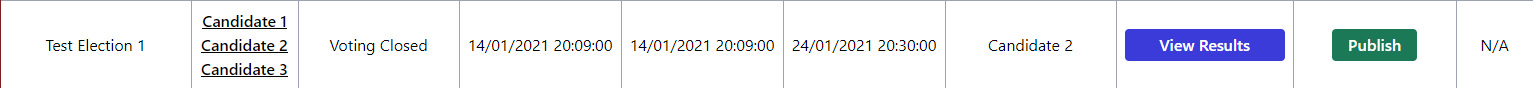
\includegraphics[width=\textwidth,height=\textheight,keepaspectratio]{elections/election_row_publish.png}
    \caption{Election results ready for publication}
    \label{fig:election_publication_ready}
\end{figure}
Just click the green 'Publish' button and the result will be viewable from the 'Elections' page that any JCR member can access. This only publishes who won and no information about the breakdown of the vote. 
\subsubsection{Revisit the Results}
You can easily return to the generated results from the main management page for the elections. Simply find the row and you'll see a blue button labelled 'View Results'. Click this to come back to the results (they won't be regenerated however, once the results are generated once they are saved for future use).
\subsubsection{Anonymous Voting Logs}
You can validate the results of the election from the results page by clicking on the green 'Load Round' button. It is strongly advised to only press one and read through it first as the log will be very long if many people have voted. It anonymises the voters and candidates but you can follow through easily.
\end{document}
